\tikzsetnextfilename{sat_hist_hom}
\begin{figure}[ht]
\centering
\begin{tikzpicture}
    \node[anchor=south west,inner sep=0] (image) at (0,0) {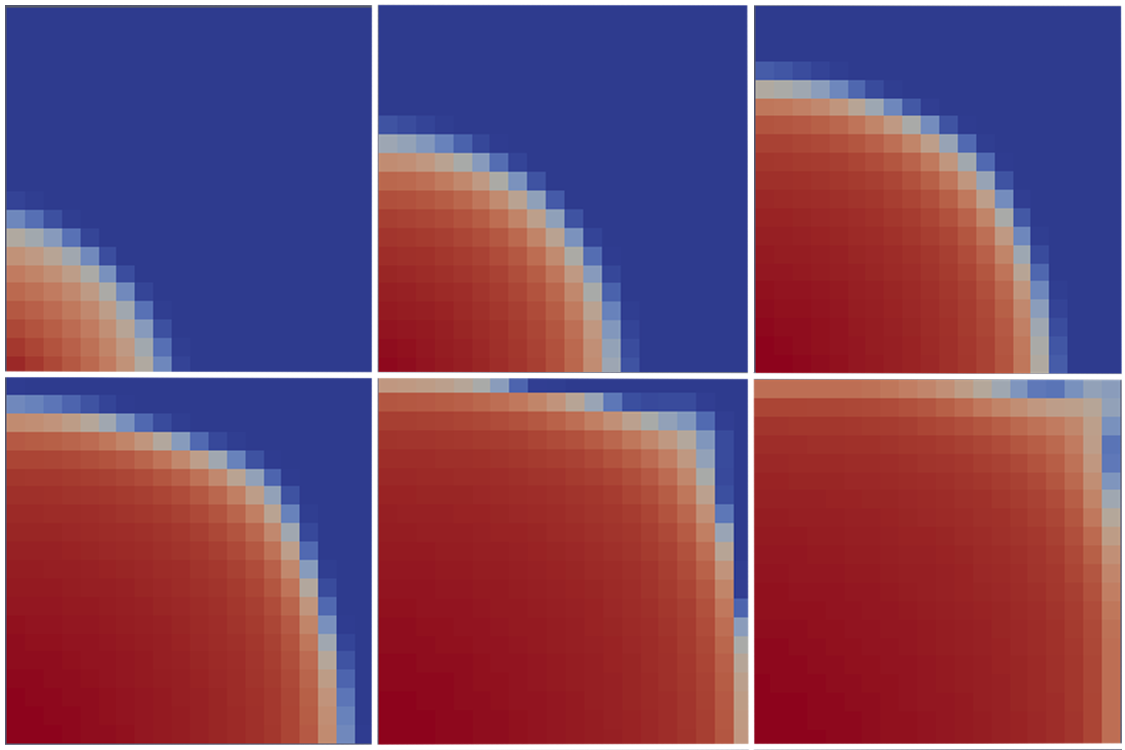
\includegraphics[width=0.6\textwidth]{figures/sat-hist-s-i-T-300-t-30-perm-10.png}};
\end{tikzpicture}
\caption{$S_w$ profile when solving the Q5 problem on a 20x20 grid with $t_{\text{end}} = \unit[300]{d}$ and $\Delta t = \unit[60]{d}$. The region has a homogeneous permeability of $\unit[10]{mD}$. Blue is oil, red is water.}
\label{fig:sat_hist_hom}
\end{figure}